\documentclass[a4paper,titlepage,fleqn,12pt]{article}

\usepackage[utf8]{inputenc}
\usepackage[T1]{fontenc}
\usepackage[english]{babel}
\usepackage{color}
\usepackage{float}
\usepackage{fancyvrb}
\usepackage{amssymb}
\usepackage{amsmath}
\usepackage{listings}

\usepackage{comment}

\usepackage{graphicx}
\usepackage{ulem}
\usepackage{pdfpages}

\DeclareGraphicsExtensions{.png}

\definecolor{dkgreen}{rgb}{0,0.45,0}
\definecolor{gray}{rgb}{0.5,0.5,0.5}
\definecolor{mauve}{rgb}{0.30,0,0.30}

\lstset{frame=tb,
  language=Java,
  aboveskip=3mm,
  belowskip=3mm,
  showstringspaces=false,
  columns=flexible,
  basicstyle={\small\ttfamily},
  numbers=left,
  numberstyle=\footnotesize,
  keywordstyle=\color{dkgreen}\bfseries,
  commentstyle=\color{dkgreen},
  stringstyle=\color{mauve},
  frame=single,
  breaklines=true,
  breakatwhitespace=false,
  tabsize=1
}


\begin{document}

\begin{titlepage}
	\begin{center}
	
\includegraphics[scale=1.5,page=7]{sdu_logos.pdf}~\\[0.5cm]
	\textsc{\Large{Syddansk Universitet - Mærsk Mc-Kinney Møller Institutet}} \\[0.2cm]
	\rule{12cm}{1pt} \\[0.4cm]
	{ \huge \bfseries Interaktion og interaktionsdesign, efterår 14, Projekt del 1 \\[0.4cm] }
	\rule{12cm}{1pt} \\[1.5cm]
	
	\begin{minipage}{0.4\textwidth}
		\begin{flushleft} \large
			\textit{Author:}\\
			Morten Rovelt Hansen\\
			Brian Pedersen\\
			Steven Gøhler\\
		\end{flushleft}
	\end{minipage}
	\begin{minipage}{0.4\textwidth}
		\begin{flushright} \large
			\textit{Supervisor:} \\
			Jess Uhre Rahbek
		\end{flushright}
	\end{minipage}
	
	\vfill
	
	{\large Oktober 10, 2014}
	\end{center}
	\newpage
\end{titlepage}

\tableofcontents
\newpage

\section{Problemfelt}

\subsection{Hvad vi vil lave}
Vi vil udarbejde en hjemmeside, der gør det nemt og brugervenligt for en jobsøgende / kommende jobsøgende, at oprette og opdaterer en online-portfolie, der er nem, hurtig og let tilgængelig at præsenterer for en arbejdgiver eller bruger.

\subsection{Antagelser}
En antagelse kunne være at hjemmesiden ikke appelerer til alle erhvervsmæssige retninger, men mest af alt kan være brugbar for folk i kreative erhverv medgør. Det ville mest være henvist til folk i mode/design/foto verdenen, da det nemme og overskuelige aspekt mest er velegnet til at bruge sammen med fremvisninger af billeder mm.

\subsection{Vil projektet have det ønskede resultat?}
Hvis realiseringen af projektet bliver ført ud med den ikke alt for tekniske og let designbare aspekt som vi rigtig gerne vil, kan enhver uden nogen form for kendskab til kodning, lave en let, flot og præsentabel portfolio, og projektet ville være en success.

\section{Hvem er brugerne?}
Vi prøver så vidt muligt at ramme en kreativ erhvervs gruppe der med henblik på design, selv skal kunne lave deres portfolie med klik fra musen uden spild tid eller kendskab til kodning. Den visuelle opsætning af siden skal appelerer til folk der hurtigt vil have en oversigt over en persons projekter, som nemt er til at skabe et overblik over.

\section{Hvad er brugernes behov?}
En nem og hurtig portfolie til at vise frem, uden at skulle lave en hel hjemmeside selv. En side hvor man kan fremvise sin kunnen, sine personlige oplysninger og ting man gerne vil have en anden person skal se, som personen hurtigt og visuelt nemt kan danne sig et overblik over.

\section{Hvilke krav stiller dette til vores løsning}
\begin{itemize}
	\item Vores side skal være nemt tilgængelig
	\item Vores layout skal være visuelt overskueligt
	\item Vores undersider skal være navnelinket
	\item Vores side skal være nemt navigerlig
	\item Vores design skal være statisk
	\item Vores side skal være fri for andet end relevante oplysninger, men stadig være visuel flot og funktionel
\end{itemize}

\section{Konceptuel model}

\begin{figure}[H]
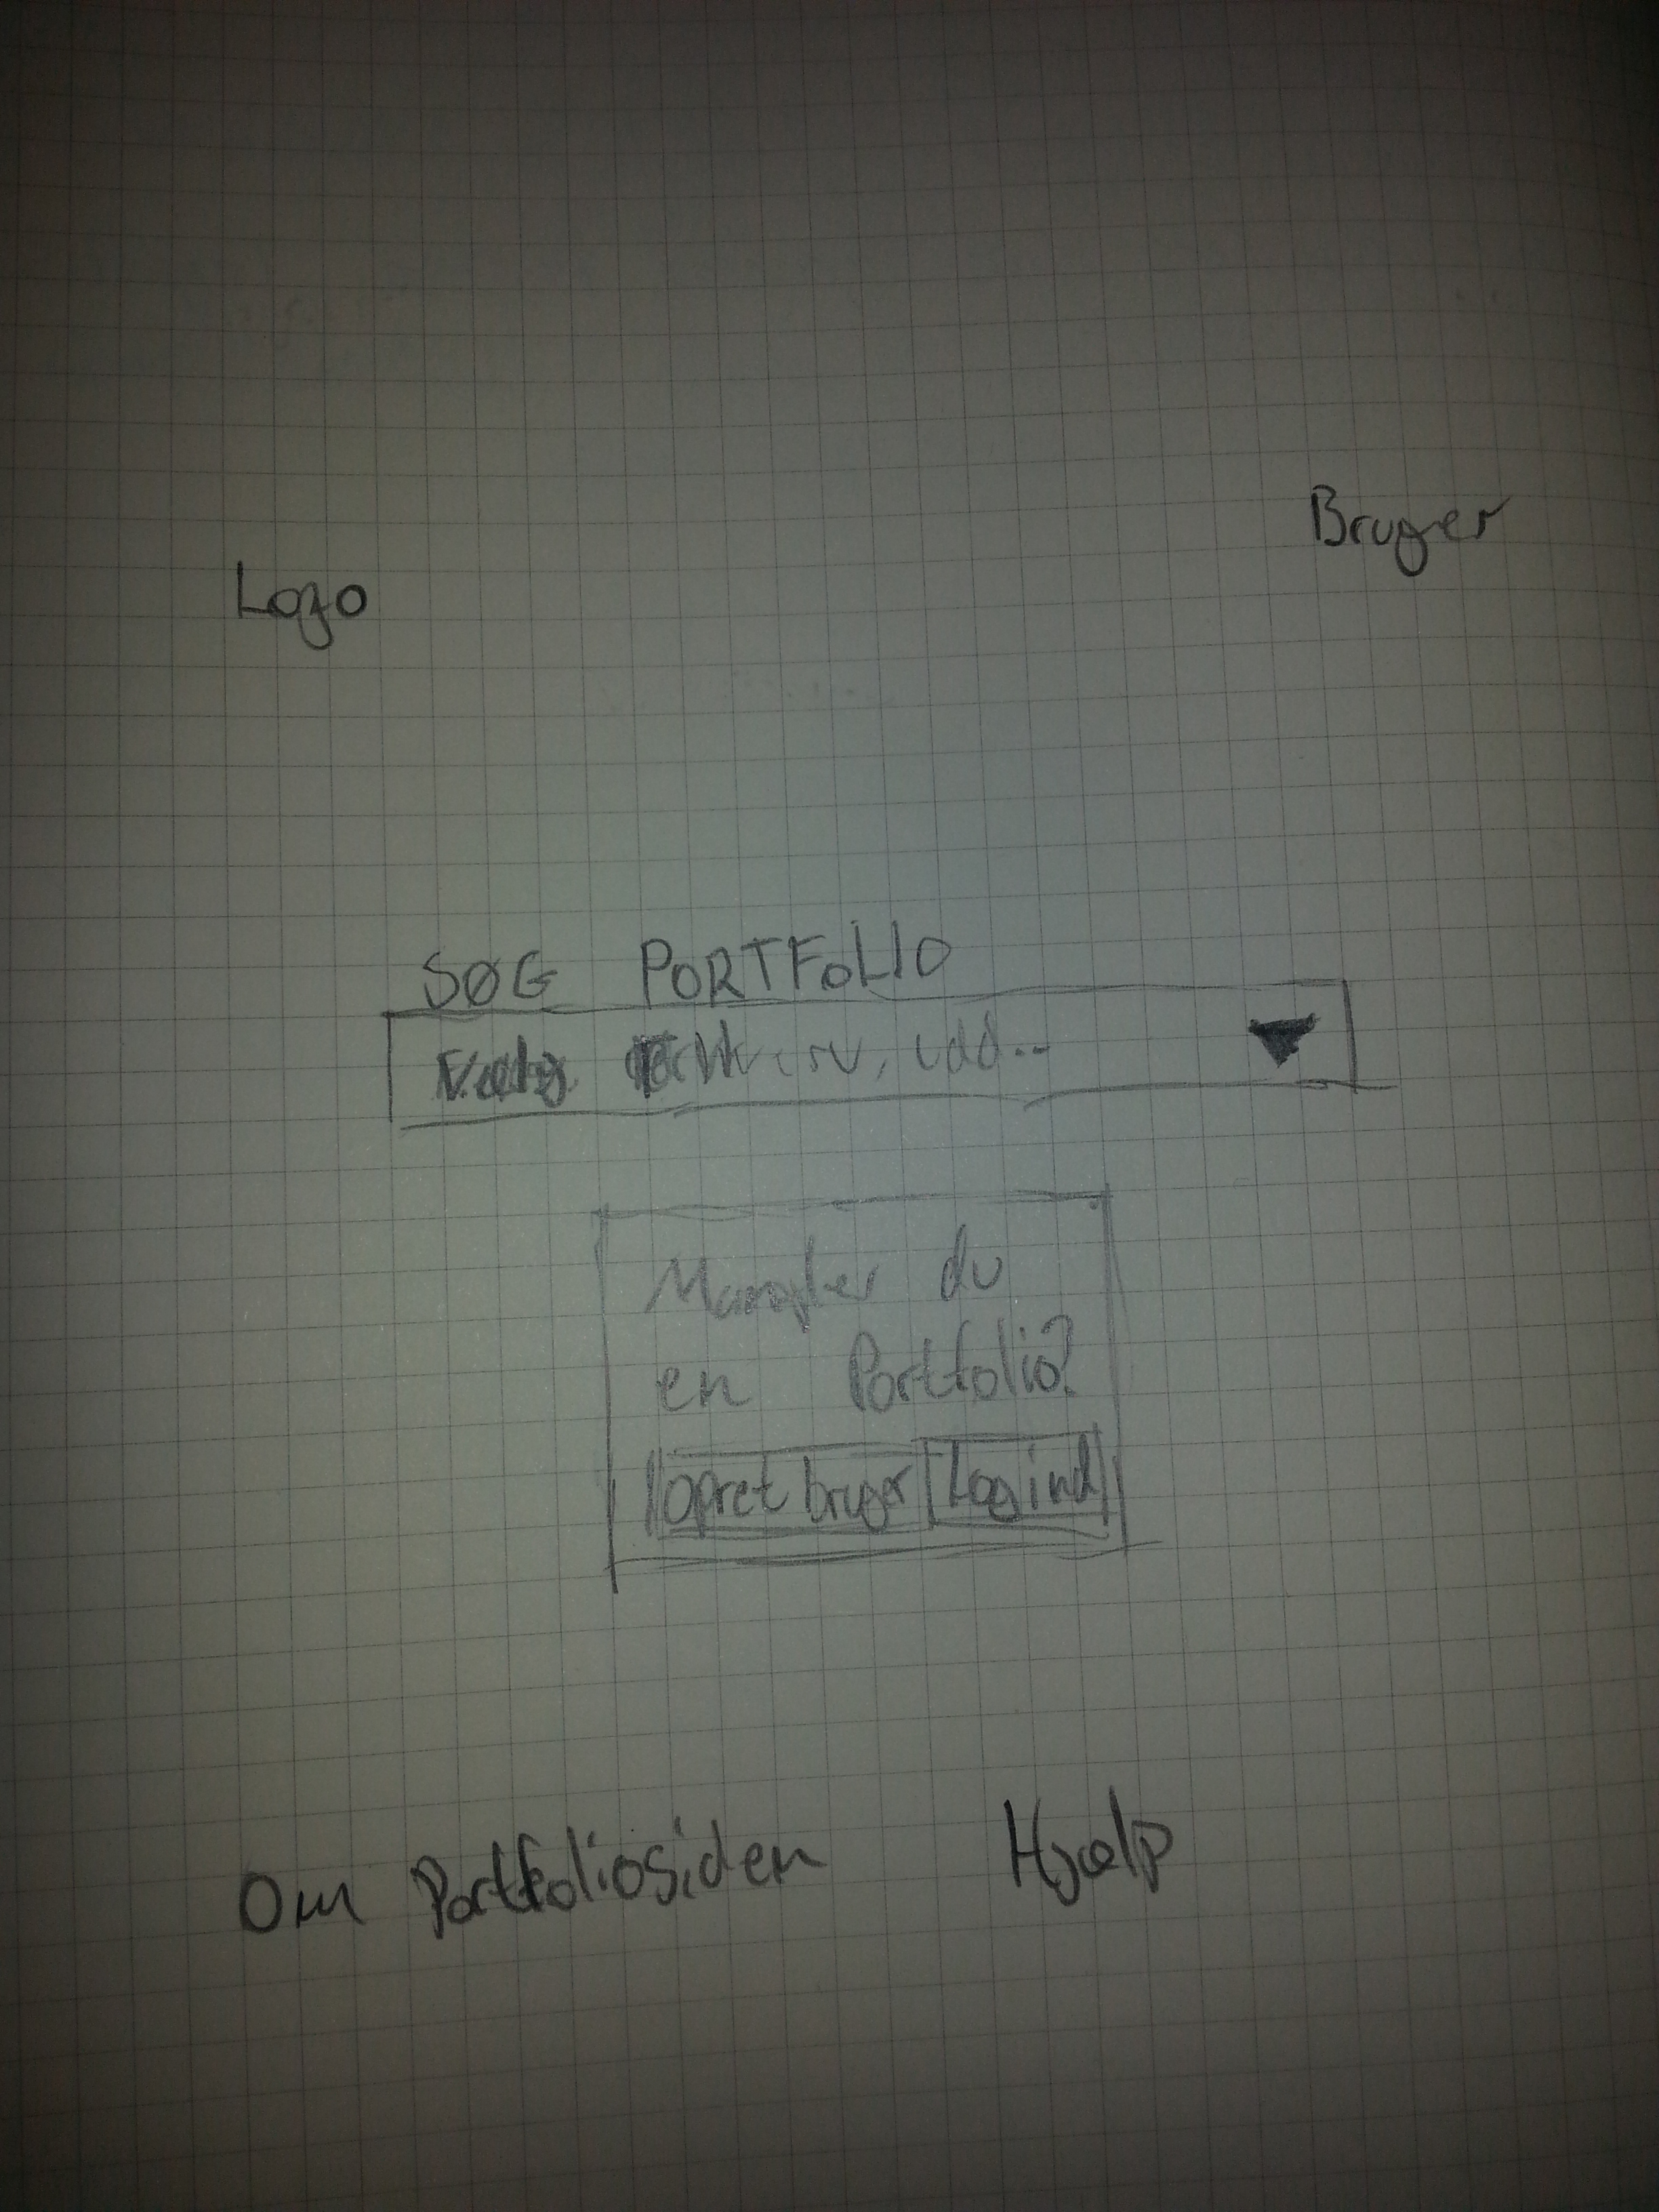
\includegraphics[width=\textwidth]{startside.jpg}
\caption{Startside hvor man kan søge på portfolier}
\end{figure}

\begin{figure}[H]
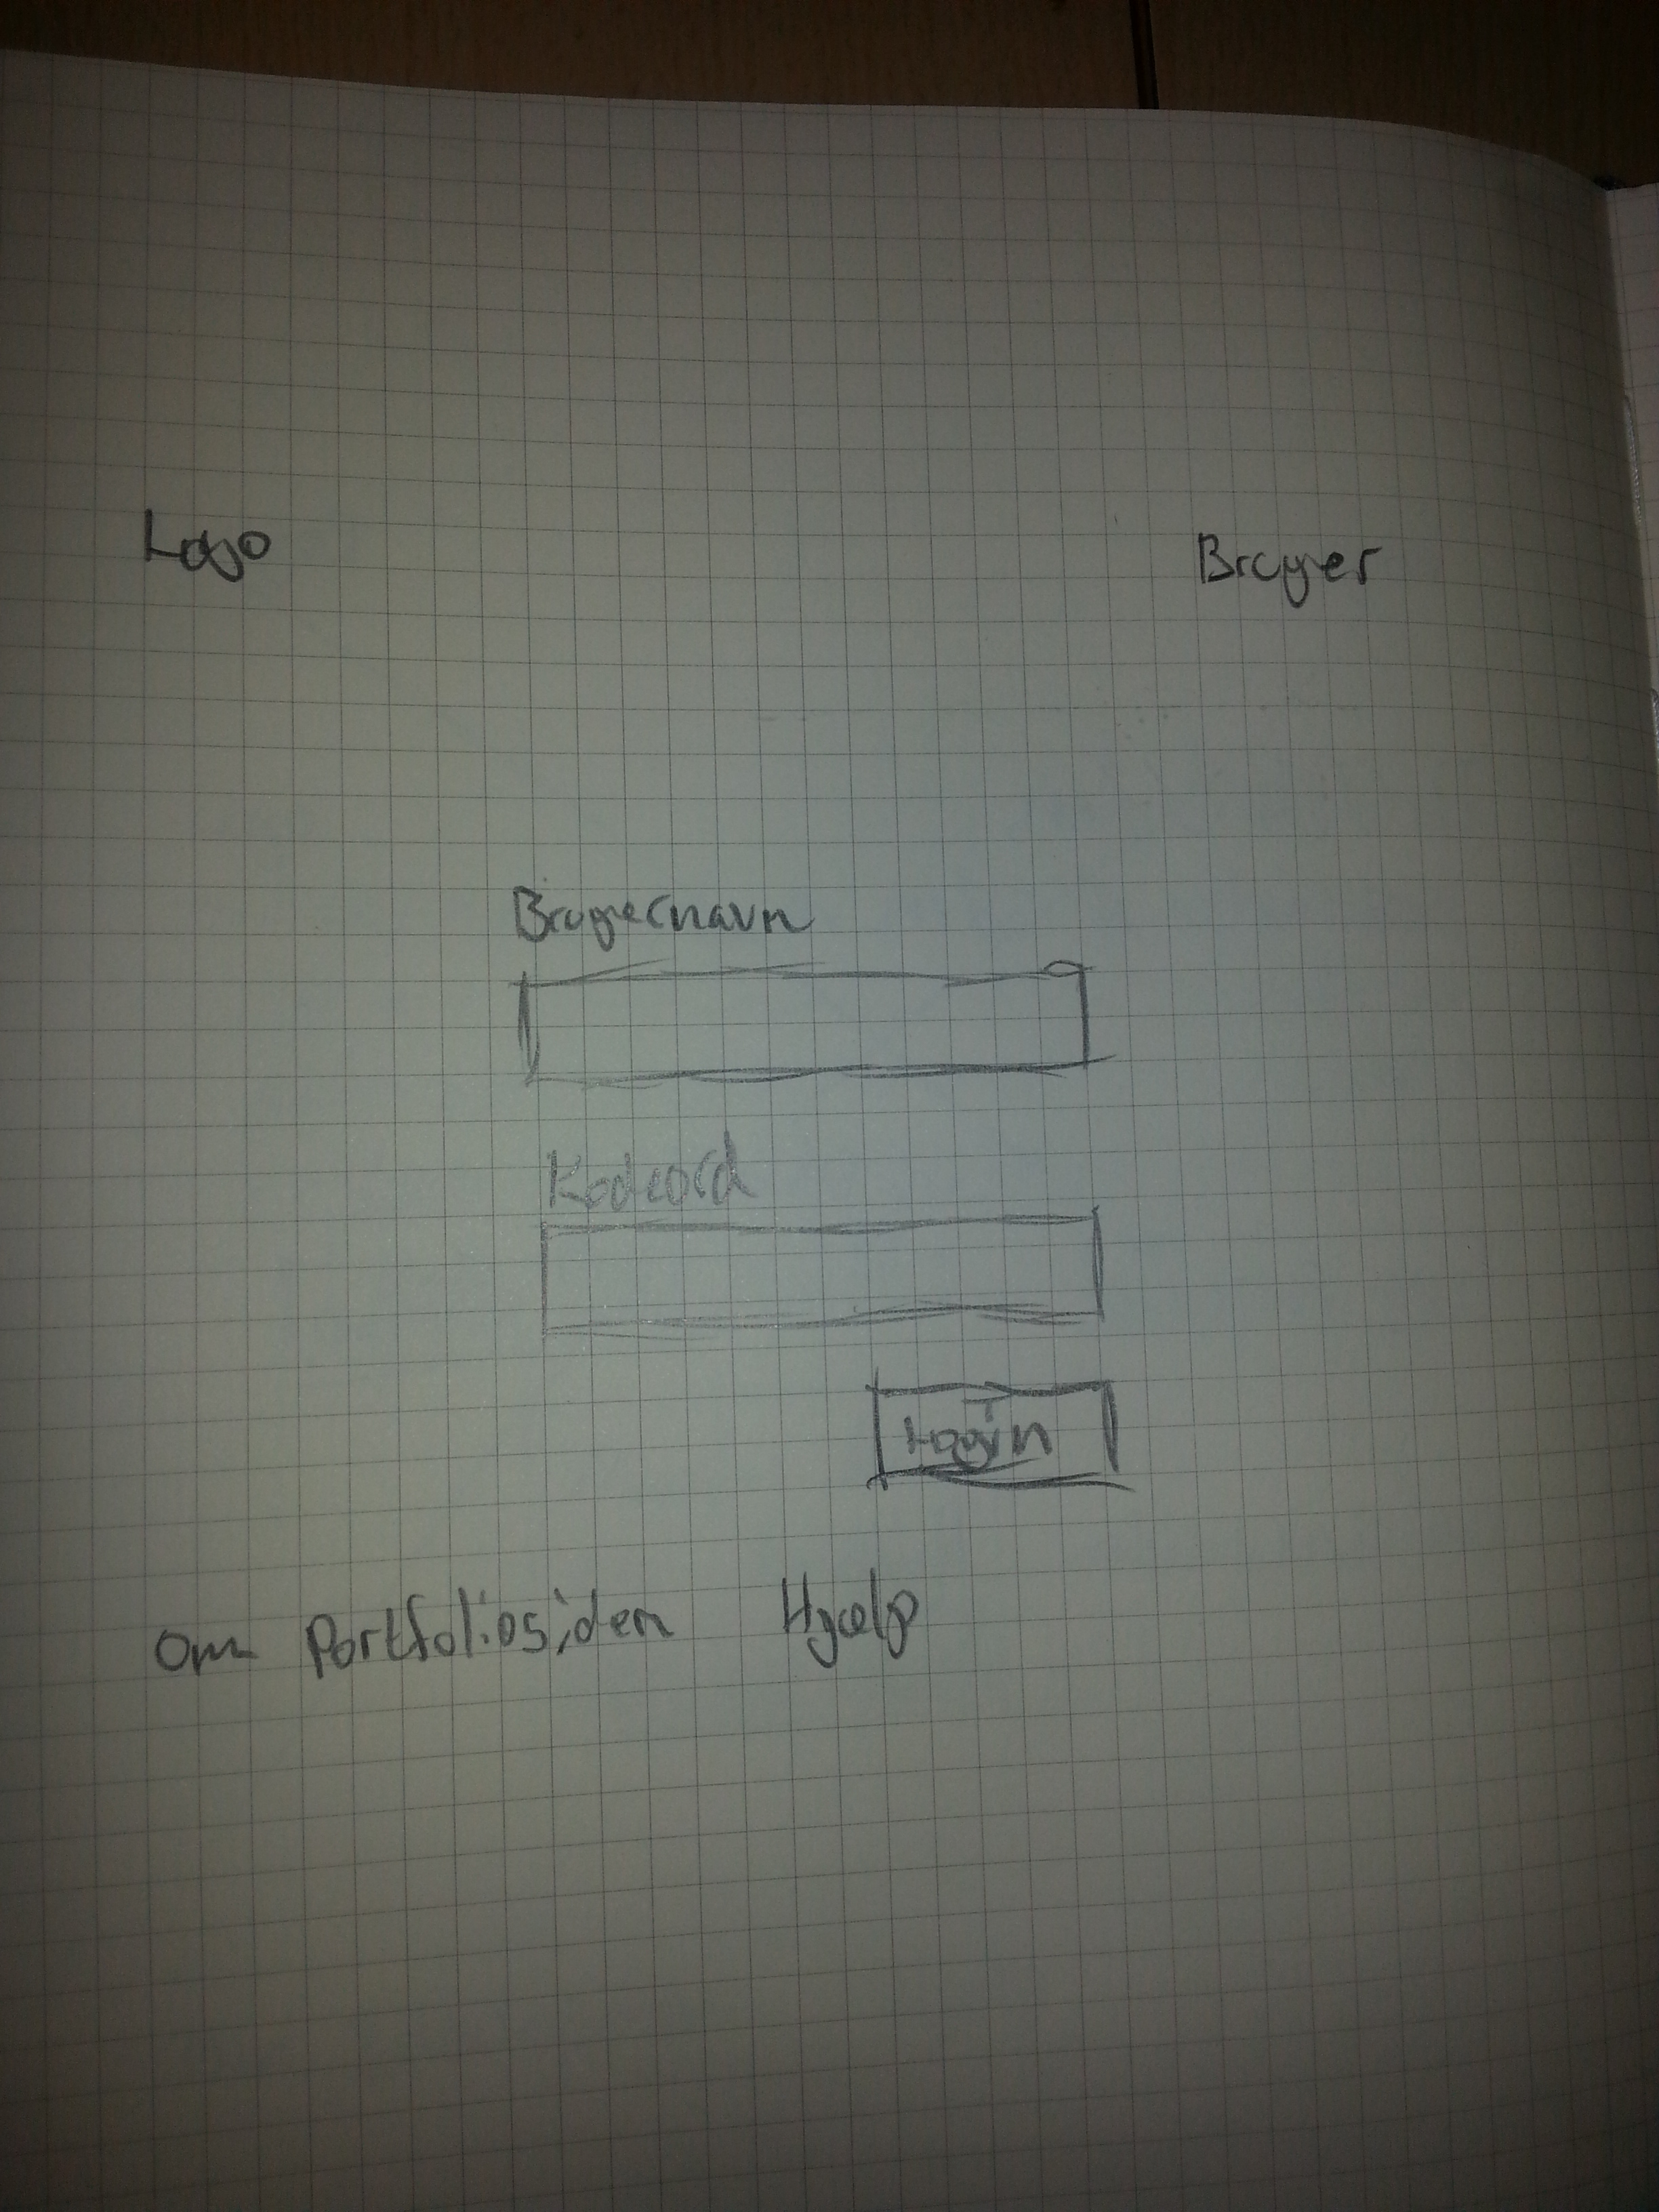
\includegraphics[width=\textwidth]{login.jpg}
\caption{Login screen hvis man har en bruger}
\end{figure}

\begin{figure}[H]
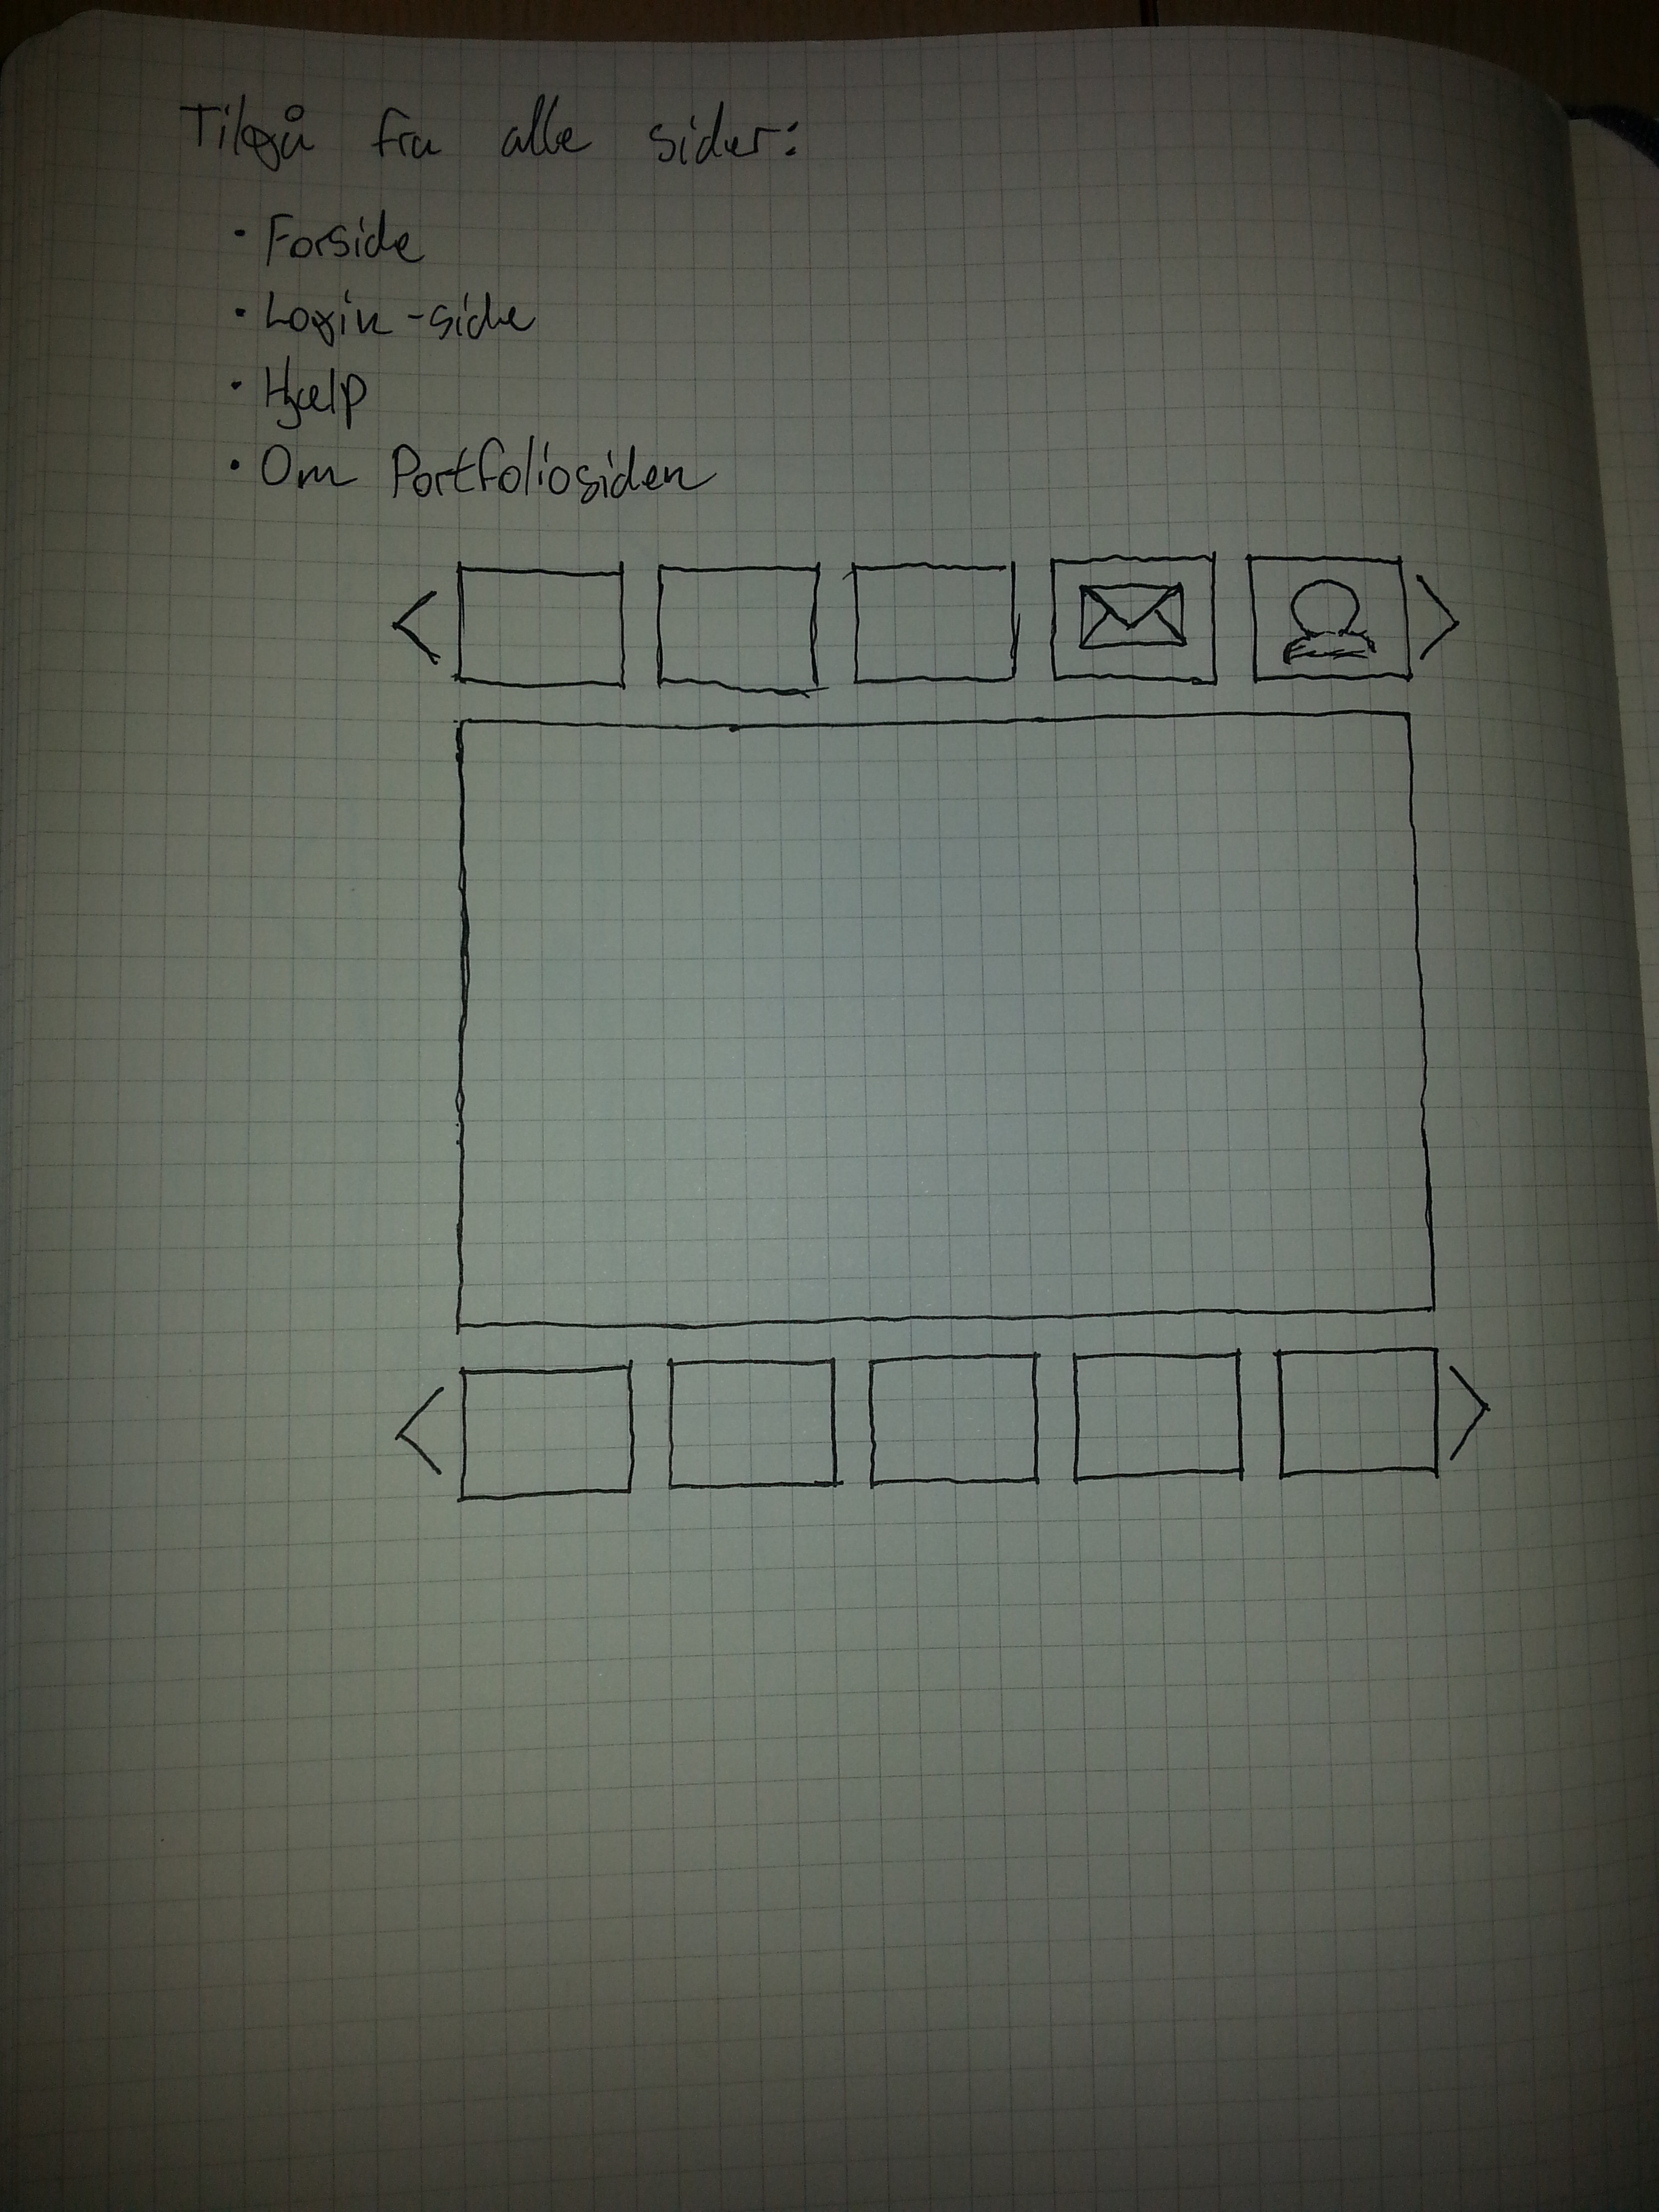
\includegraphics[width=\textwidth]{mainside.jpg}
\caption{Her ses portfilen hvor man kan tiløje og gennemse gemte projekter}
\end{figure}

\section{Personas}
\subsection{Lisa, 24 år}
\begin{description}
	\item[Beskæftigelse] Designstuderende på Århus Universitet
	\item[Teknisk følelse/attitude] glad for teknologi, og fremadrettet design mæssigt.
\end{description}
\paragraph{Baggrund}\hfill\\Lisa er en frisk ung pige der til daglig studerer på universitet, og har en bred omgangskreds. Lisa drømmer om at kunne afslutte universitet og komme ud og prøve kræfter med erhvervslivet men har ikke rigtig lavet andet erhvervsmæsigt end at sidde ved kassen i fakta. Hun bor alene i byen uden andre.

\subsection{Henning, 22 år}
\begin{description}
	\item[Beskæftigelse] Webintegrater freelance arbejder
	\item[Teknisk følelse/attitude] høj teknisk viden.
\end{description}
\paragraph{Baggrund}\hfill\\Henning er en ung og udadvendt mand, hvis liv primært drejer sig om hans arbejde. Han beskæftiger sig med freelance design og programmering af hjemmesider, hovedsagligt for mindre virksomheder. Der er dog mange om buddet på markedet, og det er meget forskelligt fra måned til måned, hvor meget arbejde han kan få. Henning er dog for nyligt flyttet sammen med hans kæreste Gertrud som arbejder på McDonalds, og de er lige i stand til at få økonomien til at løbe rundt i de måneder Henning ikke kan få så meget arbejde.

\subsection{George, 38 år}
\begin{description}
	\item[Beskæftigelse] Travl selvstændig erhvervsdrivende
	\item[Teknisk følelse/attitude] Ikke særlig teknisk anlagt og gider ikke computere
\end{description}
\paragraph{Baggrund}\hfill\\

\subsection{Betina, 45 år}
\begin{description}
	\item[Beskæftigelse] Ansættelses medarbejder i større firma
	\item[Teknisk følelse/attitude] bruger behov, bruger computer på arbejde.
\end{description}
\paragraph{Baggrund}\hfill\\

\end{document}